\documentclass[10pt,a4paper]{article}
\usepackage[utf8]{inputenc}
\usepackage[frenchb]{babel}
\usepackage[T1]{fontenc}
\usepackage{graphicx}
\usepackage{fancyhdr}

\lhead{Créer facilement son site Internet avec Wordpress}
\rhead {Rémy Mondi (iMaugis)}
\lfoot{
\includegraphics[scale=0.5]{img/cc-by-nc-sa.png}}
\cfoot{}
\rfoot{Page \thepage}

\pagestyle{fancy}

\title{Créer facilement son site Internet avec Wordpress}
\author{Rémy Mondi (iMaugis)}
\date{\today}

\begin{document}

\maketitle
\begin{figure}[!h]
\begin{center}

\includegraphics[scale=0.5]{img/logo-wordpress.png}
\end{center}
\end{figure}
\newpage

\tableofcontents
\newpage

\part*{Qu'est-ce que Wordpress?}
\addcontentsline{toc}{part}{Qu'est-ce que Wordpress?}
\newpage

\part{Installer Wordpress}
\newpage

\section{Où trouver Wordpress?}
\subsection{Télécharger Wordpress}
\paragraph{}Démarrez votre navigateur et rendez-vous à l'adresse suivante :
\paragraph{}http://fr.wordpress.org/
\begin{center}
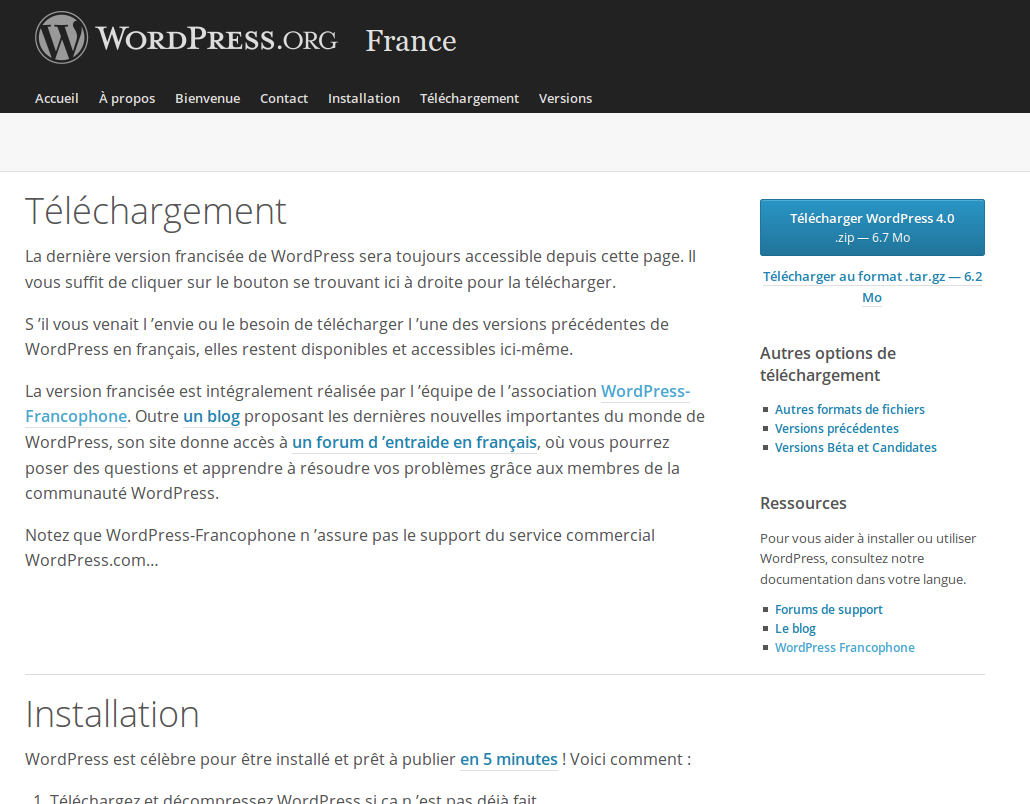
\includegraphics[scale=0.35]{img/0001.png}
\end{center}
\paragraph{}Cliquez sur le bouton « Téléchargez Wordpress X.X »
\begin{center}
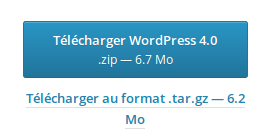
\includegraphics[scale=0.7]{img/0002.png}
\end{center}
\paragraph{}Dans la boîte de dialogue qui apparaît, sélectionnez « Enregistrer le fichier » (ou équivalent suivant votre navigateur) puis cliquez sur « Ok »
\begin{center}
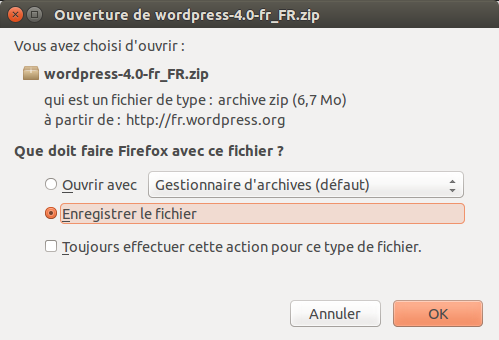
\includegraphics[scale=0.5]{img/0003.png}
\end{center}
\paragraph{}Le téléchargement se lance...
\paragraph{}Et voilà ! Vous avez téléchargé Wordpress qui doit désormais se situer dans le dossier « Téléchargements » de votre répertoire personnel sous la forme d'une archive compressée nommée wordpress-x.x-fr\_FR.zip
\subsection{Décompresser l'archive téléchargée}
\paragraph{}Rendez-vous dans le dossier « Téléchargements » de votre répertoire personnel.
\paragraph{}Faites un clic-droit sur l'archive wordpress-x.x-fr\_FR.zip puis, dans le menu contextuel qui apparaît, cliquez sur « Extraire ici ».
\begin{center}
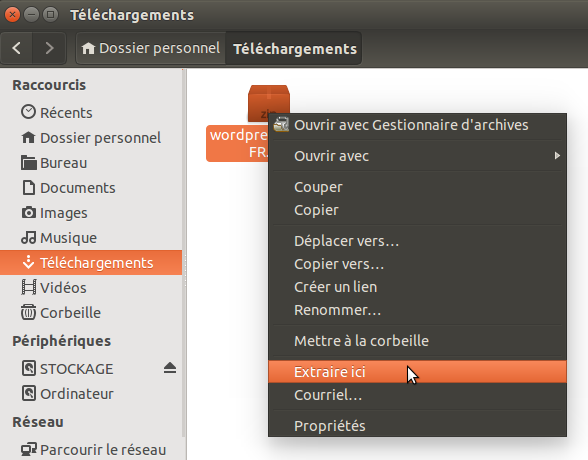
\includegraphics[scale=0.5]{img/0004.png}
\end{center}
\paragraph{}L'archive est désormais décompressée, vous pouvez observez tous les dossiers et fichiers composant Wordpress (comme ci-dessous) :
\begin{center}
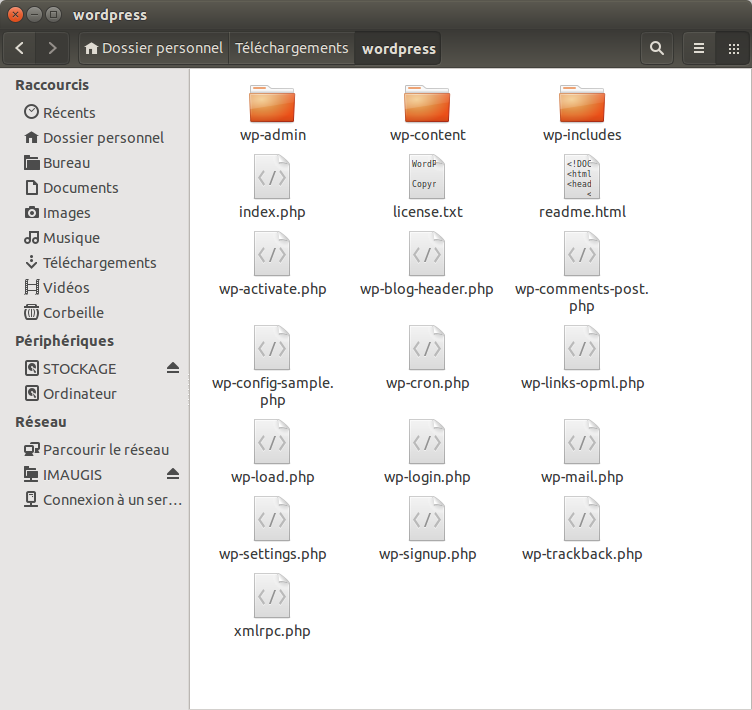
\includegraphics[scale=0.4]{img/0005.png}
\end{center}
\newpage

\section{Héberger son site Wordpress}
\subsection{Qu'est-ce qu'un hébergement?}
\paragraph{}Comme expliqué lors de la première session, tout bon site qui se respecte est « hébergé » sur un serveur. Les serveurs ne sont ni plus ni moins que des ordinateurs améliorés (matériel plus performant et plus solide) qui sont allumé 24h/24 et 7 jours / 7. Ils sont en général regroupés dans des lieux qu'on appelle des Data Center. Le rôle des serveurs est... de servir ! En l'occurrence dans notre cas de permettre à notre site Wordpress d'être accessible à tous moments par vos futurs visiteurs en entrant simplement l'adresse web du site (appelé aussi nom de domaine) ou en effectuant une recherche via un moteur de recherche (Google, Yahoo, etc...).
\begin{center}
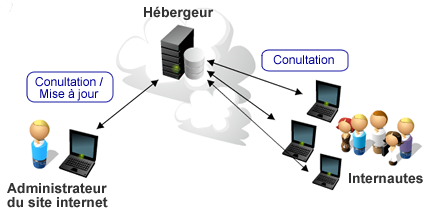
\includegraphics[scale=0.5]{img/0006.png}
\end{center}
\paragraph{}Mais louer ou mettre en place un serveur web n'est pas chose aisée et il faut des compétences spécifiques afin d'accomplir cette tâche.
\paragraph{}Heureusement pour nous, il existe une autre solution qui ne nécessite que peu de compétences : l'hébergement dit « mutualisé ».
\paragraph{}En effet un hébergement mutualisé est une parcelle allouée sur un serveur. Plusieurs sites Internet peuvent donc se partager le même serveur web (d'où le terme mutualisé).
\begin{center}
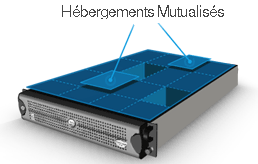
\includegraphics[scale=0.5]{img/0007.png}
\end{center}
\paragraph{}Les avantages de cette solution sont nombreux :
\begin{itemize}
\item Coûts faibles
\item Toutes les interventions techniques sont à la charge de l'hébergeur
\item Aucune connaissance d'administration requise
\item Nombreux services annexes inclus (nom de domaine, comptes email, etc...)
\end{itemize}
\paragraph{}C'est pourquoi nous vous conseillons cette solution pour héberger votre site Wordpress !
\paragraph{}Voir les offres : https://www.ovh.com/fr/hebergement-web/
\subsection{Un Hébergement mutualisé abordable : OVH}
\paragraph{}Vous trouverez chez OVH des offres d'hébergement mutualisé très fiables et tout à fait abordables pour le budget d'une association.
\begin{center}
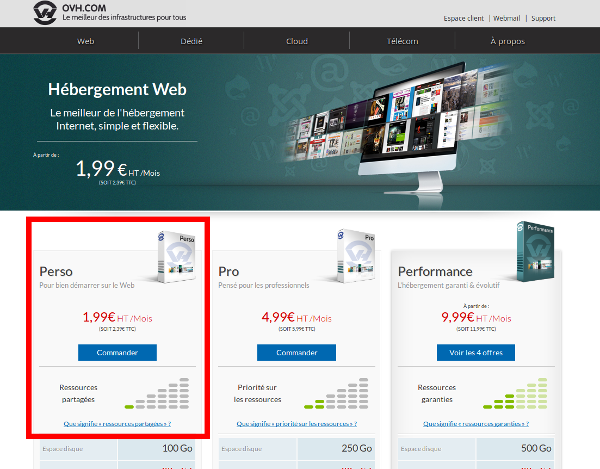
\includegraphics[scale=0.5]{img/0008.png}
\end{center}
\subsection{Comprendre les information envoyée par l'hébergeur}
\paragraph{}J'ai loué un hébergement mutualisé, que faire ensuite ?
\paragraph{}Vous avez loué un hébergement mutualisé et vous avez reçu un email avec des données étranges à l'intérieur... Nous allons apprendre à nous en servir !
\paragraph{}Voici un exemple de mail que vous recevrez :
\begin{center}
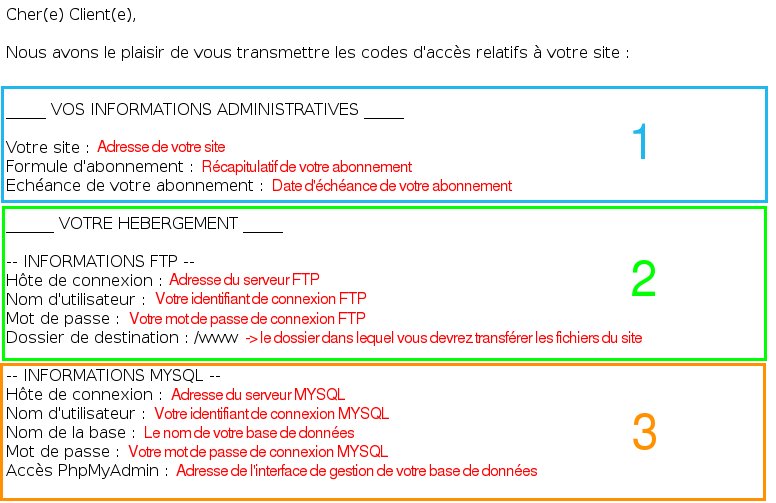
\includegraphics[scale=0.4]{img/0009.png}
\end{center}
\paragraph{}Décortiquons un peu ce mail.
\paragraph{}Première partie (encadrée en bleu) : Ce sont les données administratives. Elles rappellent simplement l'offre que vous avez choisi et la date d'échéance de celle-ci.
\paragraph{}Seconde partie (encadrée en vert) : Ce sont les données de l'espace de stockage de l'hébergement mutualisé, celui qui accueillera les fichiers de votre site Wordpress. Nous utiliserons ces données lors du transfert des fichiers de Wordpress.
\paragraph{}Troisième partie (encadrée en orange) : Ce sont les données de la base de données MYSQL que nous utiliserons lors de la procédure d'installation de Wordpress.
\newpage

\section{Transférer les fichiers de Wordpress sur un hébergement mutualisé}
\paragraph{}Nous avons, jusqu'à présent :
\begin{itemize}
\item Téléchargé Wordpress
\item Décompressé l'archive et préparé les fichiers du site
\item Choisi un hébergement mutualisé
\item Compris les données envoyées par notre hébergeur
\end{itemize}
\paragraph{}Nous sommes donc prêt à transférer les fichiers de Wordpress sur notre hébergement mutualisé !
\paragraph{}Enfin... presque...
\paragraph{}Le transfert des fichiers ne se fait pas par email ni par magie, il nous faut utiliser un logiciel spécifique et adapté à ce genre de tâche : un client FTP

\subsection{Qu'est-ce qu'un client FTP?}
\paragraph{}Un client FTP est un logiciel qui, comme son nom l'indique, utilise le protocole FTP qui signifie Protocole de Transfert de Fichier (File Transfer Protocole en Anglais). Il permet donc, depuis un ordinateur, de copier des fichiers vers un autre ordinateur (un serveur par exemple...). Il permet aussi d'administrer un site web ou encore de supprimer ou modifier des fichiers sur cet ordinateur.
\begin{center}
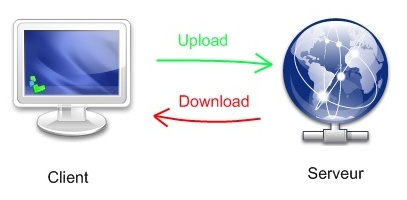
\includegraphics[scale=0.7]{img/0010.jpg}
\end{center}

\subsection{Un client FTP libre et gratuit: FileZilla}
\begin{center}

\includegraphics[scale=0.1]{img/0011.png}
\end{center}
\paragraph{}FileZilla est un client FTP puissant et complet. Il a l'avantage d'être libre et gratuit mais aussi multi-plateforme c'est à dire qu'il fonctionne aussi bien sous Windows que sous Linux et MacOs.
\paragraph{}Nous choisirons donc ce logiciel pour transférer les fichiers de 
Wordpress sur votre hébergement mutualisé.
\subsubsection{Installer FileZilla sous Microsoft Windows}
\paragraph{}Démarrez votre navigateur et rendez-vous à l'adresse suivante :
\paragraph{}http://filezilla-project.org/
\paragraph{}Une fois sur le site, cliquez sur « Download FileZilla Client » pour accéder à la page de téléchargement
\begin{center}
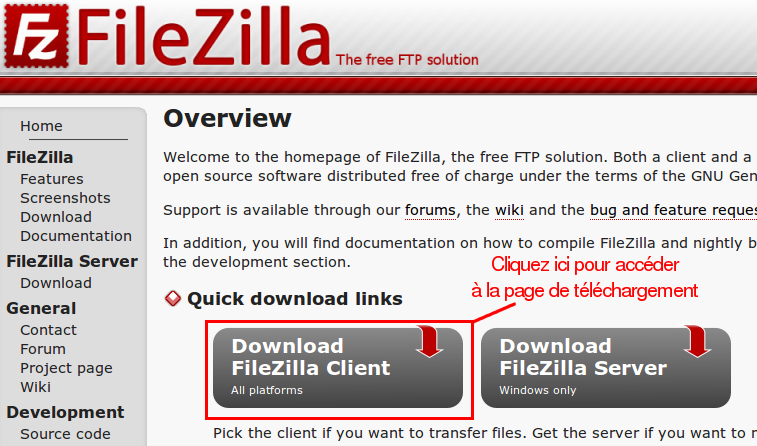
\includegraphics[scale=0.5]{img/0012.png}
\end{center}
\paragraph{}Une fois sur la page de téléchargement, cliquez sur « FileZilla\_x.x.x\_winXX-setup.exe » pour lancer le téléchargement du fichier d'installation de FileZilla
\begin{center}
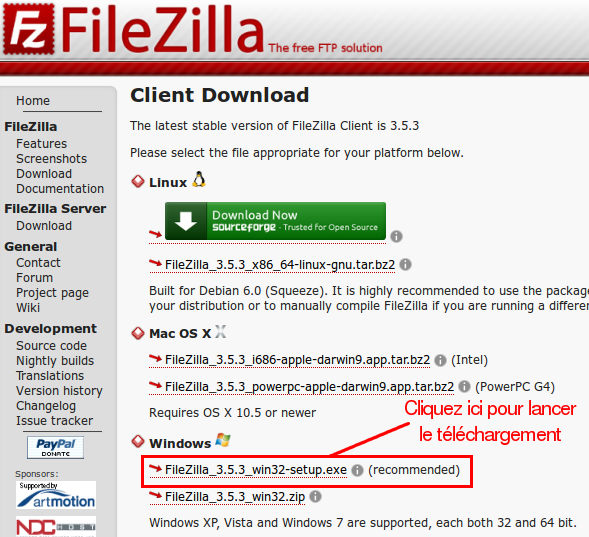
\includegraphics[scale=0.4]{img/0013.png}
\end{center}
\paragraph{}Dans la boîte de dialogue qui apparaît, sélectionnez « Enregistrer le fichier » (ou équivalent suivant votre navigateur) puis cliquez sur « Ok »
\begin{center}
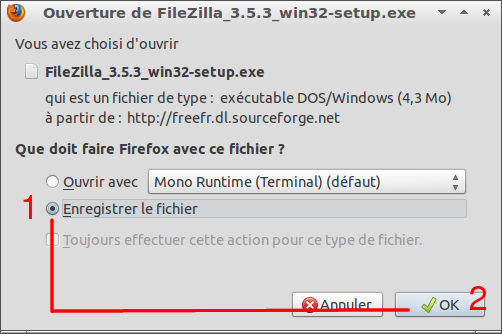
\includegraphics[scale=0.5]{img/0014.png}
\end{center}
\paragraph{}Le téléchargement se lance...
\begin{center}
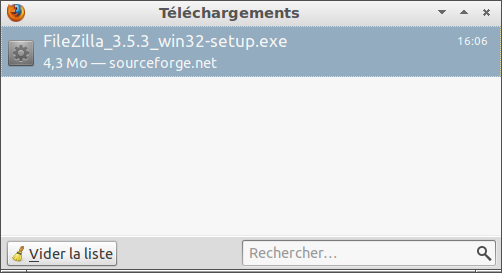
\includegraphics[scale=0.5]{img/0015.png}
\end{center}
\paragraph{}Rendez-vous dans le dossier Téléchargement situé dans votre répertoire personnel
\paragraph{}Double-cliquez sur le fichier « FileZilla\_x.x.x\_winXX-setup.exe » pour commencer l'installation du logiciel.
\paragraph{}\textbf{Étape 1 : }Licence d'utilisation
\paragraph{}Acceptez la licence d'utilisation en cliquant sur « I Agree »
\begin{center}
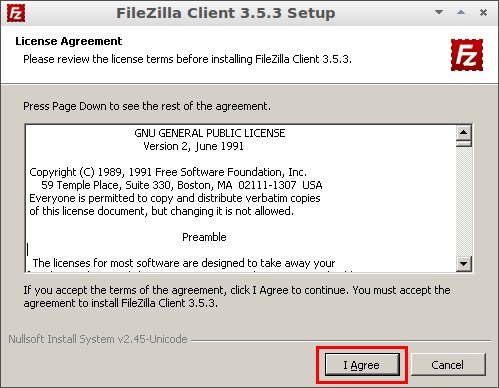
\includegraphics[scale=0.5]{img/0016.png}
\end{center}
\paragraph{}\textbf{Étape 2 : }Choix des options d'installation
\paragraph{}Sélectionnez qui aura accès à FileZilla sur votre ordinateur
\begin{itemize}
\item \textit{Anyone who use this computer (All users)} : Tous les utilisateurs pourront utiliser FileZilla
\item \textit{Only for me (Votre nom d'utilisateur)} : En cochant cette case, seul vous pourrez utilisez FileZilla
\end{itemize}
\begin{center}
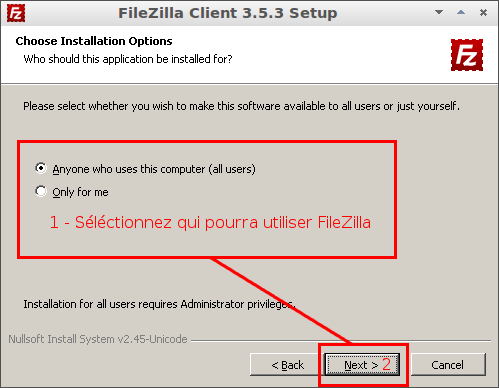
\includegraphics[scale=0.5]{img/0017.png}
\end{center}
\paragraph{}\textbf{Étape 3 : }Choix des composants
\paragraph{}Cochez la case « Desktop Icon » si vous souhaitez créer un raccourcis de FileZilla sur votre bureau. Cliquez ensuite sur « Next » pour poursuivre
\begin{center}
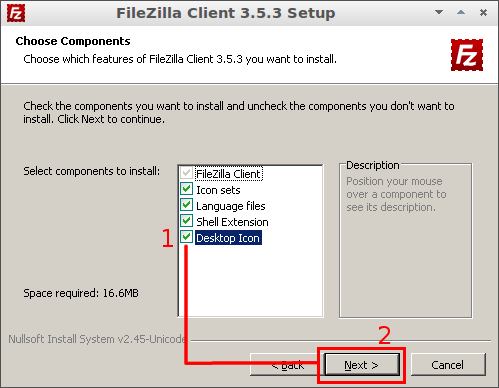
\includegraphics[scale=0.5]{img/0018.png}
\end{center}
\paragraph{}\textbf{Étape 4 : }Choix du répertoire d'installation
\paragraph{}Laissez le répertoire d'installation par défaut et cliquez « Next » pour poursuivre
\begin{center}
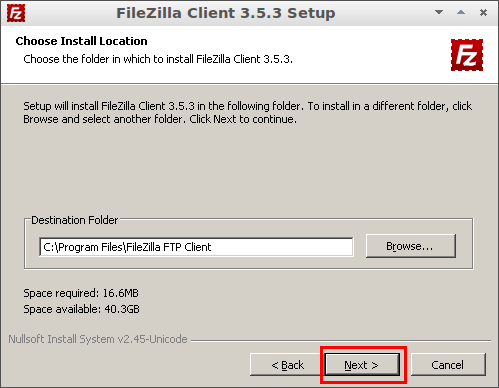
\includegraphics[scale=0.5]{img/0019.png}
\end{center}
\paragraph{}\textbf{Étape 5 : }Choix du dossier du menu Démarrer
\paragraph{}Laissez le choix par défaut puis cliquez sur «Install » pour lancer l'installation
\begin{center}
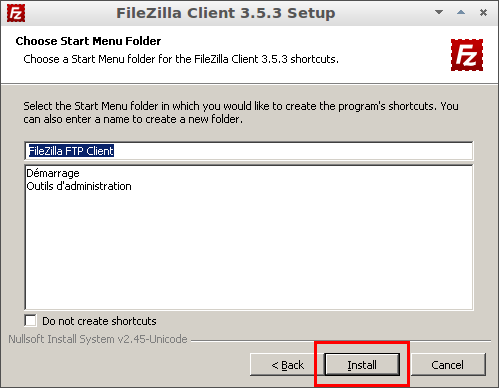
\includegraphics[scale=0.5]{img/0020.png}
\end{center}
\paragraph{}\textbf{Étape 6 : }L'installation est en cours...
\begin{center}
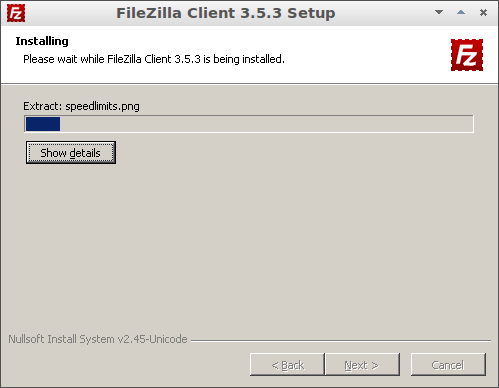
\includegraphics[scale=0.5]{img/0021.png}
\end{center}
\paragraph{}\textbf{Étape 7 : }L'installation est terminée
\paragraph{}L'installation est terminée, cochez la case « Start FileZilla nox » et cliquez sur « Finish » pour démarrer FileZilla
\begin{center}
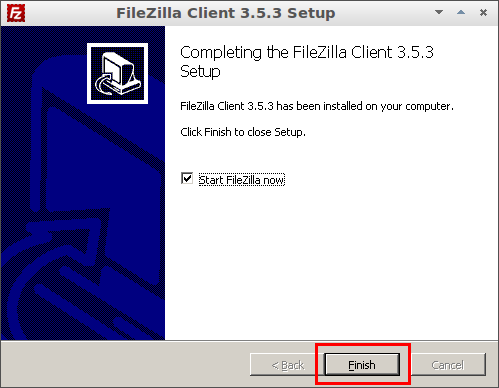
\includegraphics[scale=0.5]{img/0022.png}
\end{center}
\subsubsection{Installer FileZilla sous Linux Ubuntu}
\paragraph{}\textbf{Étape 1 : }Lancez la logithèque
\paragraph{}Lancez la logithèque
\begin{center}
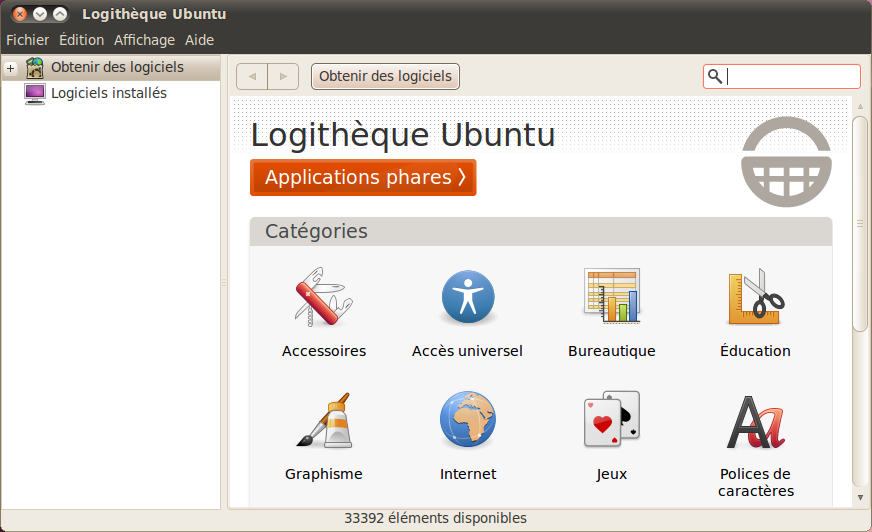
\includegraphics[scale=0.4]{img/0023.png}
\end{center}
\paragraph{}\textbf{Étape 2 : }Rechercher et installer FileZilla
\paragraph{}Recherchez Filezilla puis cliquez sur « Installer »
\begin{center}
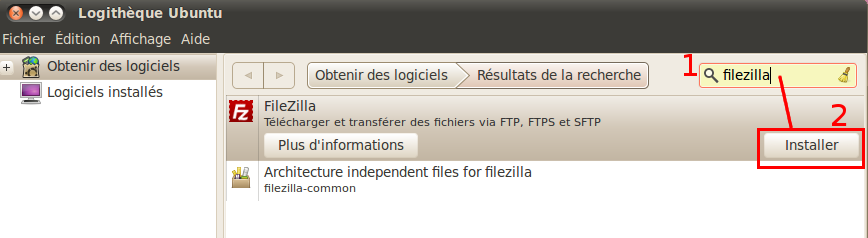
\includegraphics[scale=0.4]{img/0024.png}
\end{center}
\paragraph{}\textbf{Étape 3 : }Authentification
\paragraph{}Indiquez votre mot de passe super-utilisateur (ou root) puis cliquez sur «S'authentifier» pour lancer l'installation
\begin{center}
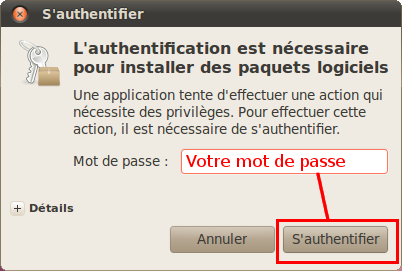
\includegraphics[scale=0.4]{img/0025.png}
\end{center}
\paragraph{}\textbf{Étape 4 : }Installation en cours...
\paragraph{}L'installation de FileZilla est en cours...
\begin{center}
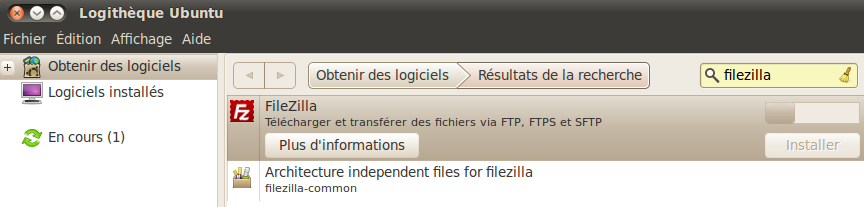
\includegraphics[scale=0.4]{img/0026.png}
\end{center}
\paragraph{}\textbf{Étape 5 : }Installation terminée
\paragraph{}L'installation est terminée !
\begin{center}
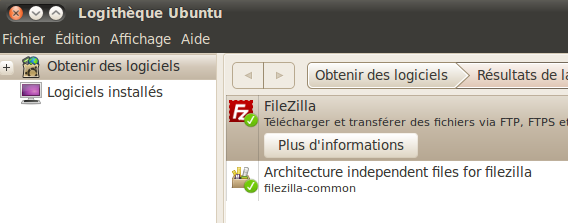
\includegraphics[scale=0.4]{img/0027.png}
\end{center}
\paragraph{}\textbf{Étape 6 : }Démarrer FileZilla
\paragraph{}Démarrez FileZilla en cliquant sur Applications > Internet > FileZilla
\begin{center}
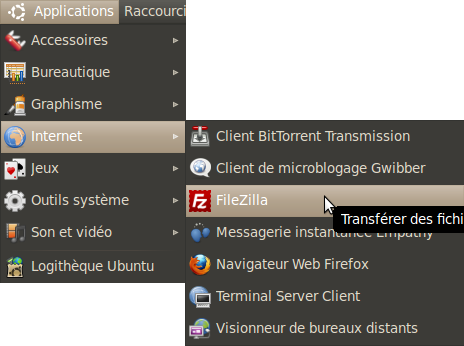
\includegraphics[scale=0.4]{img/0028.png}
\end{center}

\subsection{Tour d'horizon de FileZilla}
\subsubsection{Premier démarrage}
\paragraph{}Au premier lancement de FileZilla apparaît une boîte de dialogue vous indiquant notamment des liens vers de la documentation. Cliquez sur « Ok » pour fermer cette boîte de dialogue.
\begin{center}
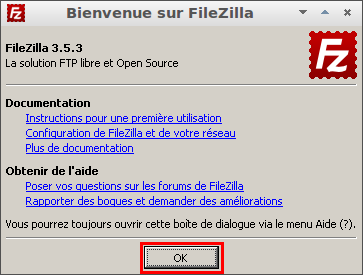
\includegraphics[scale=0.4]{img/0029.png}
\end{center}
\subsubsection{Décryptage de l'interface}
\paragraph{}Vous pouvez voir que la fenêtre principale de FileZilla est est divisée en plusieurs parties
\begin{center}
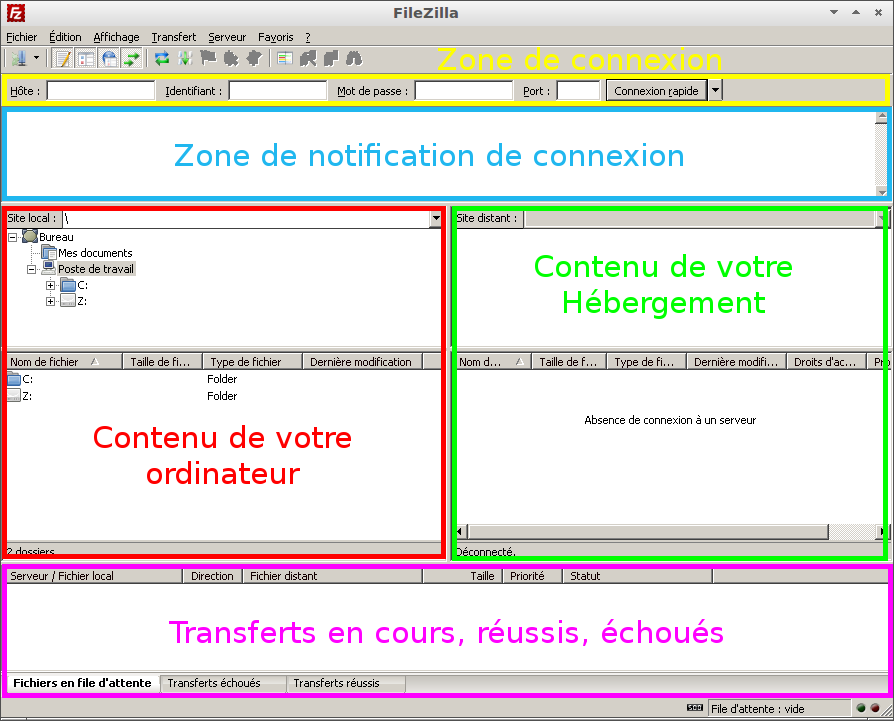
\includegraphics[scale=0.4]{img/0030.png}
\end{center}
\paragraph{}\textbf{Première partie (encadrée en jaune) :} La zone d'identification, c'est dans celle-ci que nous allons renseigner les informations de connexion pour accéder à l'espace de stockage que vous trouverez dans le mail que vous enverra votre hébergeur (voir ci-dessous).
\begin{center}
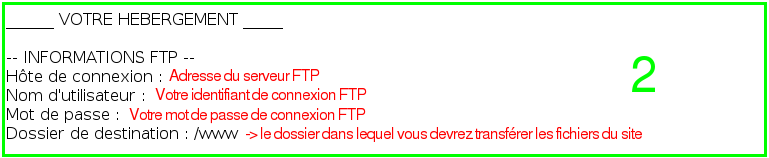
\includegraphics[scale=0.4]{img/0031.png}
\end{center}
\paragraph{}\textbf{Seconde partie (encadrée en bleu) :} La zone de notification de connexion. Vous y trouverez des informations concernant la connexion à votre hébergement (par exemple :connexion au serveur réussie ou échouée).
\paragraph{}\textbf{Troisième partie (encadrée en rouge) :} Le contenu de votre ordinateur. Affiche l'arborescence de votre ordinateur afin d'aller rechercher les fichiers à transférer sur votre hébergement.
\paragraph{}\textbf{Quatrième partie (encadrée en vert) :} Le contenu de votre hébergement (ou espace de stockage). Affiche l'arborescence de votre hébergement.
\paragraph{}\textbf{Cinquième partie (encadrée en rose) :} La zone de notification de transfert. Affiche les transferts en cours mais aussi leur statut (réussis ou échoués).

\subsection{Transférer les fichiers du site Wordpress sur l'hébergement Mutualisé}
\paragraph{}Nous sommes (enfin...) prêts à transférer les fichiers de Wordpress sur l'hébergement mutualisé.
\subsubsection{Connexion au serveur FTP}
\paragraph{}Si ce n'est pas déjà fait, démarrez FileZilla
\paragraph{}Indiquez dans la zone de connexion les informations FTP envoyées par votre hébergeur
\begin{center}

\includegraphics[scale=0.4]{img/0032.png}
\end{center}
\begin{enumerate}
\item Indiquez l'adresse du serveur FTP
\item Indiquez votre identifiant de connexion FTP
\item Indiquez votre mot de passe de connexion FTP
\item Indiquez le port FTP (sauf indication contraire de votre hébergeur, le port FTP est « 21 »)
\end{enumerate}
\paragraph{}Cliquez ensuite sur le bouton « Connexion rapide » pour vous connecter à votre hébergement mutualisé.
\paragraph{}Si tout s'est bien passé (pas de message d'erreur dans la zone de notification de connexion) vous devriez voir le contenu de votre hébergement à droite de l'écran (encadré en rouge ci-dessous)
\begin{center}
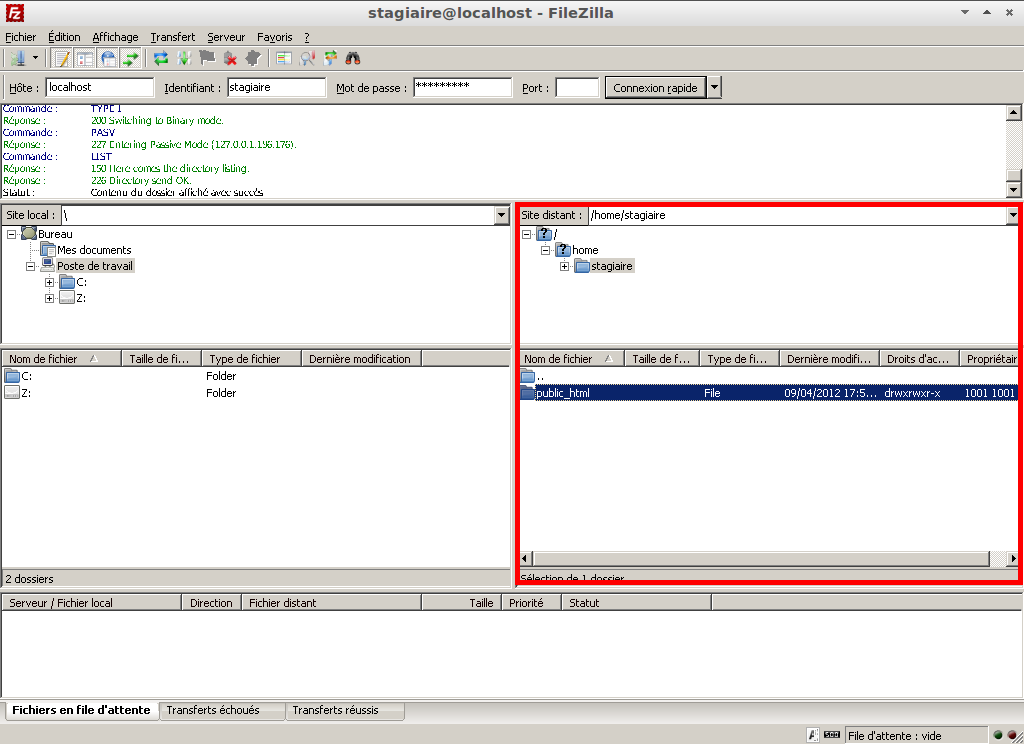
\includegraphics[scale=0.35]{img/0033.png}
\end{center}
\paragraph{}Pour le moment seul un répertoire (ici public\_html) s'y trouve. Selon votre hébergeur, ce répertoire peut s'appeler \textbf{www}, \textbf{public\_html} ou encore \textbf{web}. C'est dans ce répertoire que  vous devrez transférer les fichiers de Wordpress afin qu'ils soient visibles sur Internet.
\subsubsection{Transfert des fichiers}
\paragraph{}Double-cliquez sur le répertoire public\_html afin d'afficher son contenu
\begin{center}
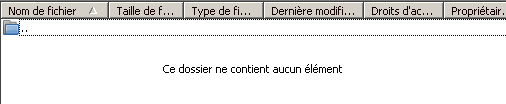
\includegraphics[scale=0.5]{img/0034.png}
\end{center}
\paragraph{}Pour le moment, il est vide...
\paragraph{}Dans la zone de contenu de votre ordinateur (encadrée en rouge ci-dessous) affichez les dossiers et fichiers de Wordpress que vous avez télécharger tout à l'heure (qui doivent normalement se situer dans le dossier Téléchargements de votre répertoire personnel)
\begin{center}
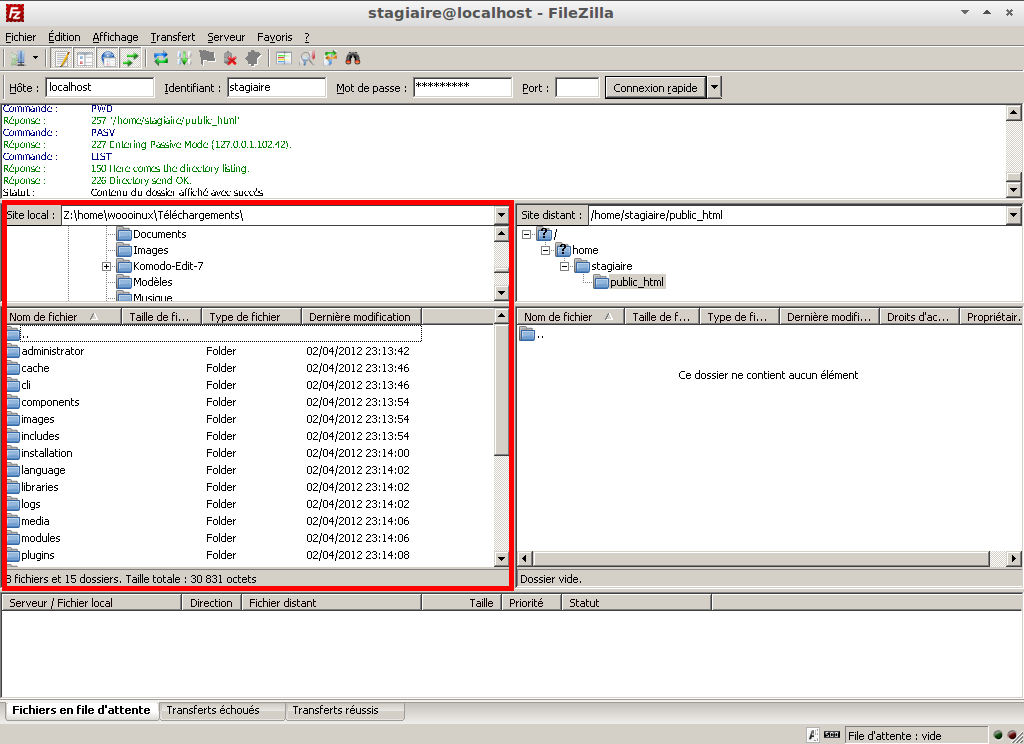
\includegraphics[scale=0.35]{img/0035.png}
\end{center}
\paragraph{}Sélectionnez tous les dossiers et fichiers puis faites un glisser-déposer vers le dossier public\_html de votre hébergement mutualisé
\begin{center}
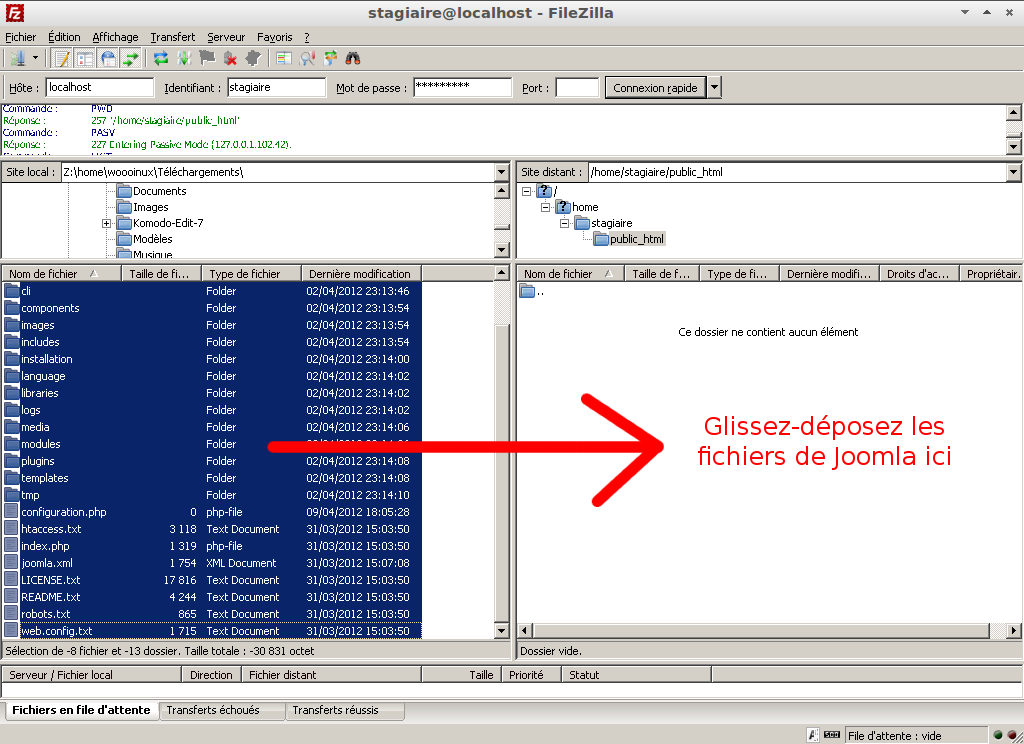
\includegraphics[scale=0.35]{img/0036.png}
\end{center}
\paragraph{}Le transfert des fichiers est en cours. Vous pouvez voir la progression et l'état du transfert dans la zone de notification des transferts (encadrée en rouge ci-dessous) et les fichiers apparaître dans le contenu de votre hébergement (encadré en vert ci-dessous)
\begin{center}
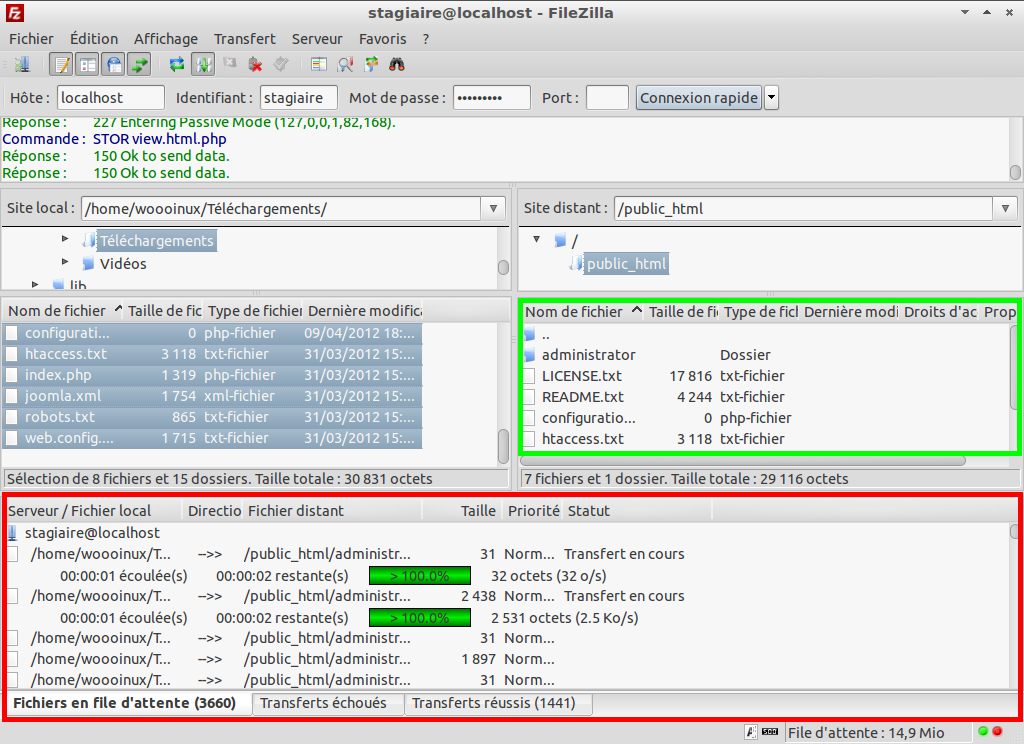
\includegraphics[scale=0.35]{img/0037.png}
\end{center}
\paragraph{}Si tout s'est bien passé (pas d'erreurs dans l'onglet Transferts échoués de la zone de notification des transferts) vous devriez voir tous les dossiers et fichiers de Wordpress dans le zone de contenu de votre hébergement (encadrée en rouge ci-dessous)
\begin{center}
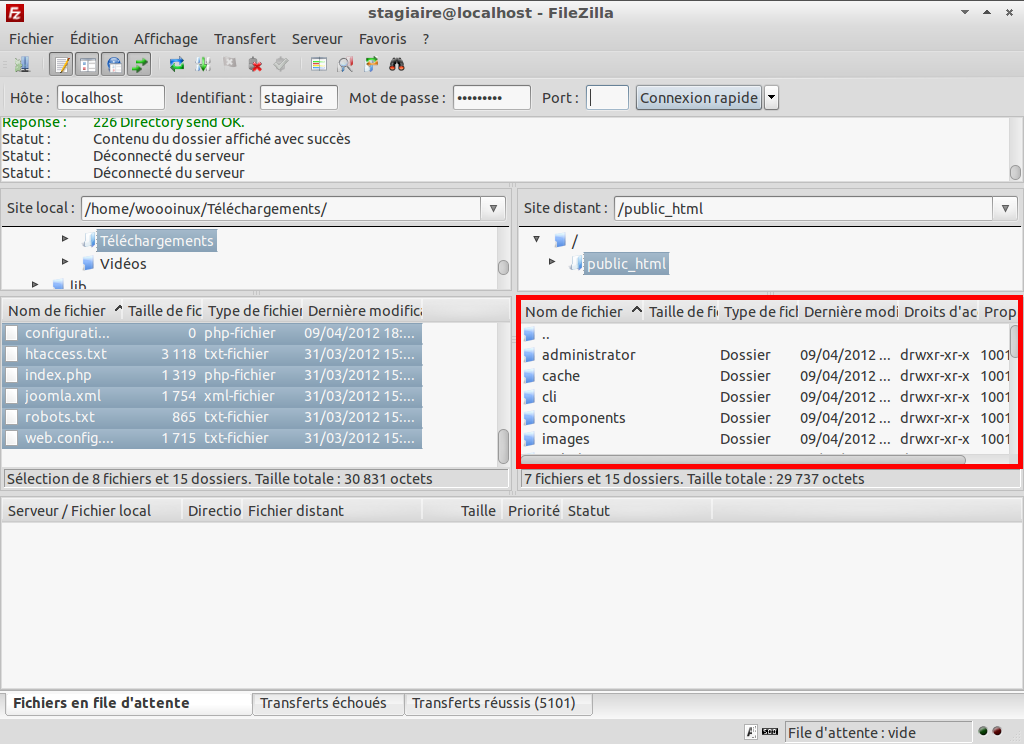
\includegraphics[scale=0.35]{img/0038.png}
\end{center}
\paragraph{}Vous pouvez maintenant quitter FileZilla
\begin{center}
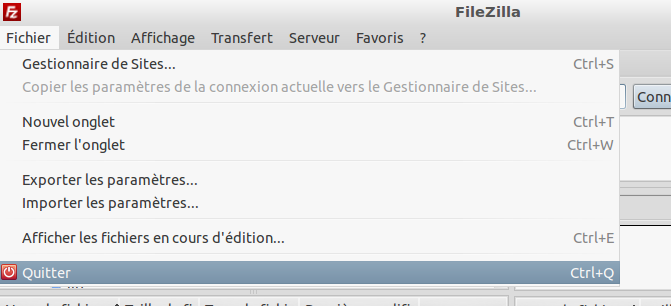
\includegraphics[scale=0.35]{img/0039.png}
\end{center}
\paragraph{}Nous avons maintenant terminé le transfert des fichiers Wordpress sur votre hébergement mutualisé, il en nous reste plus qu'à nous rendre sur le site afin de terminer l'installation.
\newpage

\section{Installer Wordpress}
\paragraph{}Accédez à votre site Wordpress en indiquant l'adresse fournie par votre hébergeur dans votre navigateur.
\paragraph{}Vous arrivez sur la page d'installation de Wordpress.
\paragraph{}\textbf{Étape 1 : }Avant propos
\paragraph{}Cette page récapitule toutes les informations dont vous aurez besoin pour mener l'installation jusqu'au bout. Si vous avez toutes ces informations, cliquez sur le bouton « C'est parti ! » pour lancer l'installation de Wordpress.
\begin{center}
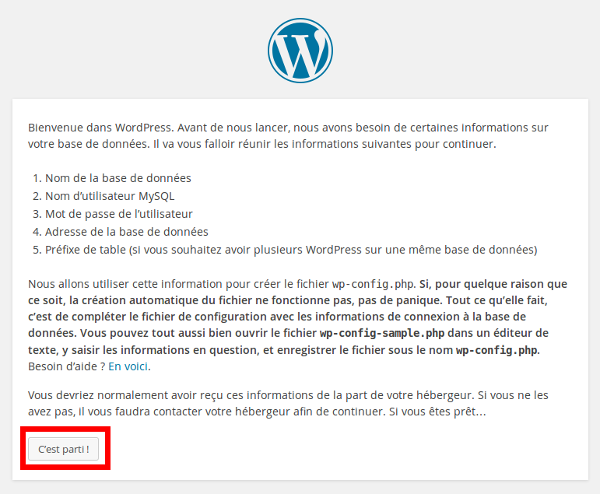
\includegraphics[scale=0.5]{img/0040.png}
\end{center}
\paragraph{}\textbf{Étape 2 : }Configuration de la base de données
\paragraph{}Cette étape est cruciale ! Vous devez indiquer les informations relatives à votre base de données afin que Wordpress puisse s'y connecter et y créer les tables dont il aura besoin.
\paragraph{}Par exemple voici comment remplir ce formulaire avec les informations que vous avez reçu lors de la formation (remplacer le « X » par votre numéro de stagiaire) :
\begin{center}
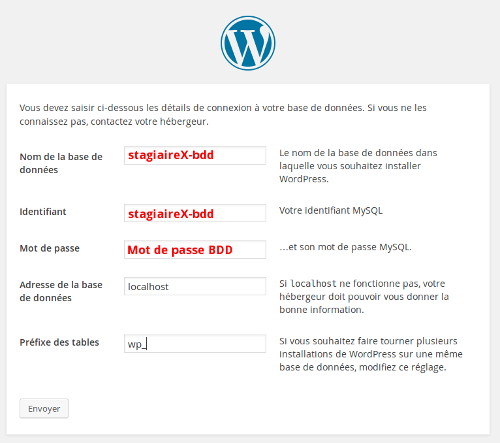
\includegraphics[scale=0.5]{img/0041.png}
\end{center}
\paragraph{}\textbf{Étape 3 : }Lancement de l'installation
\paragraph{}Si vous avez correctement renseigné les informations de connexion à votre base de données vous devriez arrivé sur une page vous disant que Wordpress est désormais capable de communiquer avec cette dernière. Cliquez sur le bouton « Lancer l 'installation » pour… lancer l'installation !
\begin{center}
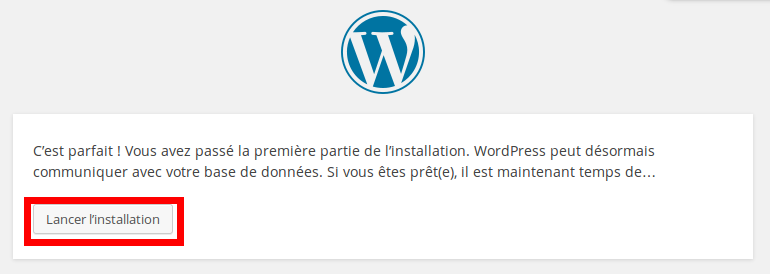
\includegraphics[scale=0.5]{img/0042.png}
\end{center}
\paragraph{}\textbf{Étape 4 : }Configuration de Wordpress
\paragraph{}Cette étape va vous permettre de configurer Wordpress. Vous allez donc donner un nom à votre site (le nom de votre structure par exemple), vous choisir un identifiant ainsi qu'un mot de passe pour accéder à l'administration et ainsi gérer votre site et enfin renseigné votre courriel.
\begin{center}
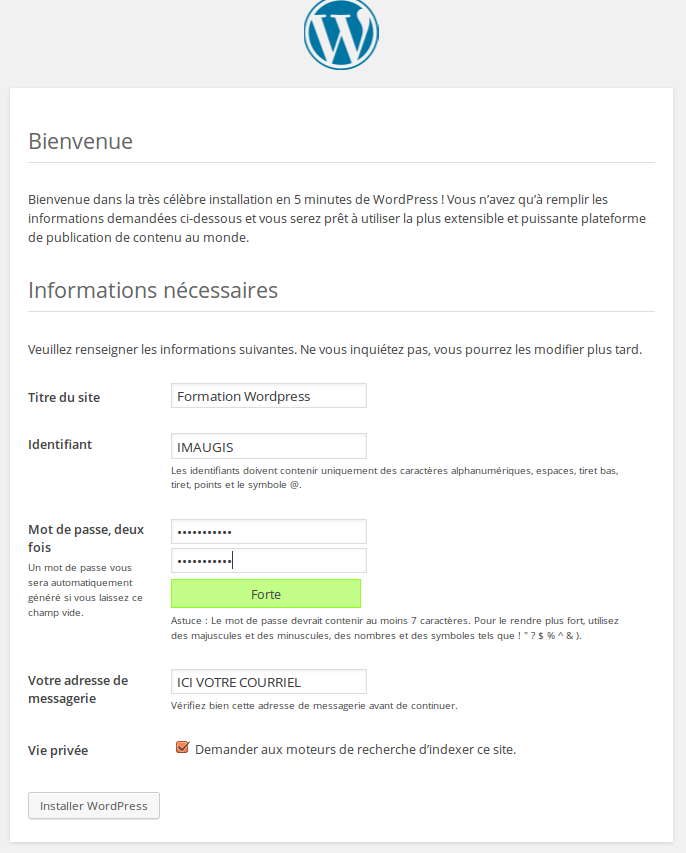
\includegraphics[scale=0.5]{img/0043.png}
\end{center}
\paragraph{}\textbf{Étape 5 : }Installation terminée
\paragraph{}Si l'installation de Wordpress s'est bien déroulée vous devriez voir apparaître une message de succès vous proposant aussi de vous connecter au back-office. Cliquez sur le bouton « Connexion » pour accéder au formulaire d'authentification :
\begin{center}
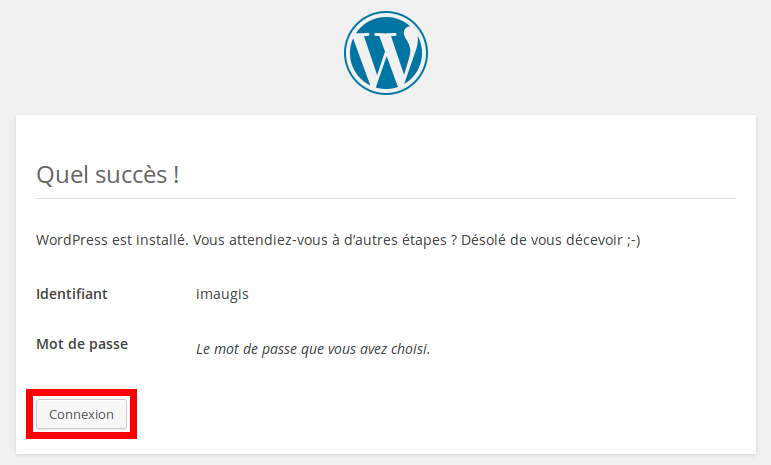
\includegraphics[scale=0.5]{img/0044.png}
\end{center}
\paragraph{}\textbf{Étape 6 : }Formulaire d'authentification
\paragraph{}Saisissez l'identifiant ainsi que le mot de passe choisis lors de l'installation (cf étape 4) et cliquez sur le bouton « Connexion ».
\begin{center}
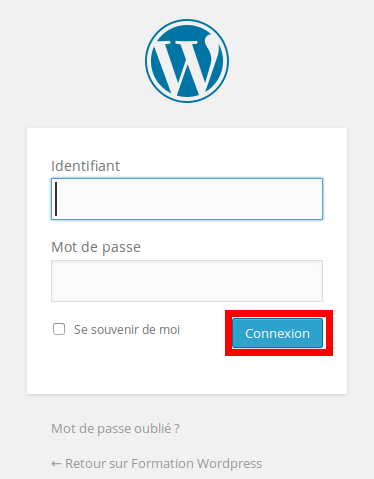
\includegraphics[scale=0.5]{img/0045.png}
\end{center}
\paragraph{}\textbf{Étape 7 : }Le Back-Office
\paragraph{}Si votre authentification s'est déroulée sans encombre vous devez arrivé sur le back-office de Wordpress. Félicitation ! L'installation de Wordpress est terminée !
\begin{center}
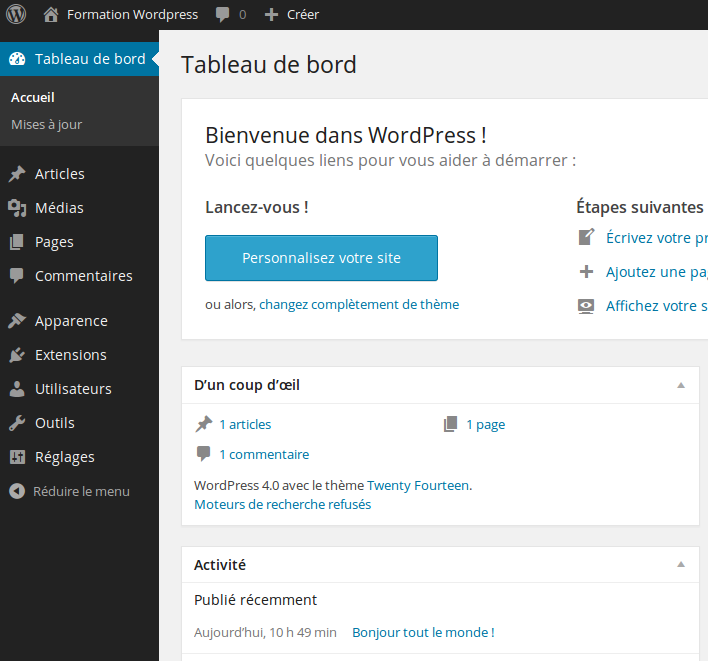
\includegraphics[scale=0.5]{img/0046.png}
\end{center}
\newpage

\part{Premiers pas avec Wordpress}
\newpage

\section{Tour d'horizon de Wordpress}
\paragraph{}Wordpress se décompose en deux partie principales : le front-office et le back-office.
\subsection{Le "Front-Office"}
\paragraph{}Le front-office est la partie site, la boutique, ce que voient les visiteurs qui viennent sur votre site.
\begin{center}
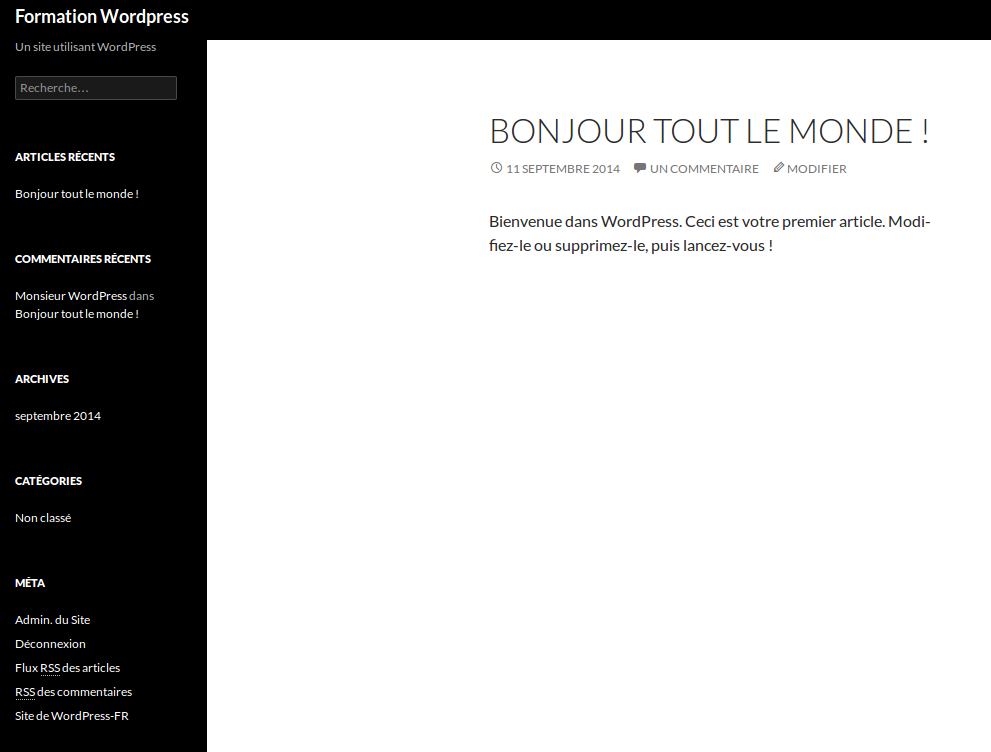
\includegraphics[scale=0.35]{img/0047.png}
\end{center}
\paragraph{}Le front-office affichera ce que vous aurez envie d'afficher c'est vous qui décidez !
\paragraph{}Par exemple : Vos articles, vos menus, vos galeries photos, vos vidéos, un forum de discussion, des sondages, etc...
\paragraph{}Pour accéder au front-office, il suffit d'entrer l'adresse de votre site (celle que vous aura communiquer votre hébergeur) dans la barre d'adresse de votre navigateur.
\paragraph{}Par exemple : http://www.monsite.com

\subsection{Le "Back-Office"}
\paragraph{}Le back-office est la partie administration. C'est l’arrière-boutique de votre site ; l'interface d’administration va permettre de créer et mettre à jour vos articles mais aussi de gérer tout votre site.
\begin{center}
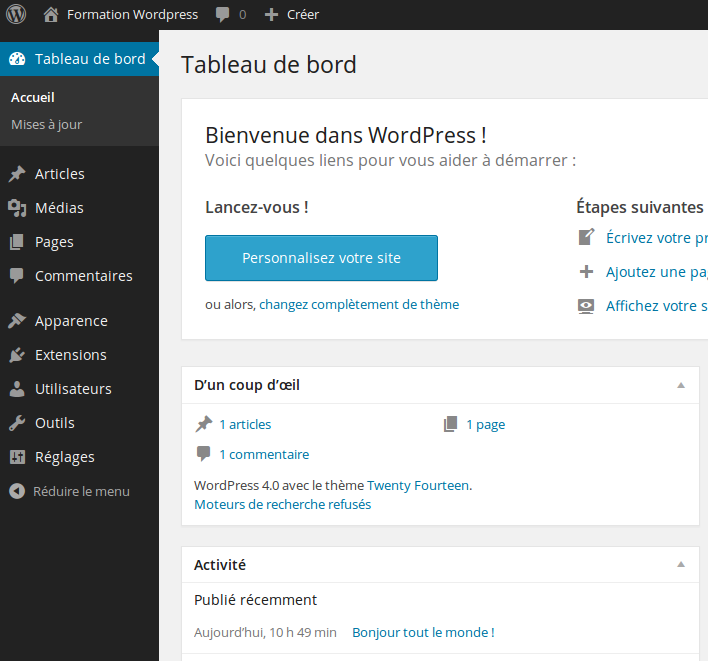
\includegraphics[scale=0.5]{img/0046.png}
\end{center}
\paragraph{}Comme expliqué plus haut, le back-office vous permettra de gérer le site :
\begin{itemize}
\item Ajouter, modifier, supprimer des articles
\item Créer des catégories pour organiser vos articles
\item Ajouter du contenu multimédia (images, sons)
\item Ajouter, modifier, supprimer des menus
\item Gérer les utilisateurs
\item D'ajouter des plugins, widgets et donc des fonctionnalités supplémentaires à Wordpress
\item De gérer le thème (design) du site
\item De mettre à jour Wordpress
\end{itemize}
\paragraph{}Pour accéder au back-office, il suffit d'entrer l'adresse de votre site suivi de « /wp-admin »
\paragraph{}Par exemple : http://www.monsite.com/wp-admin
\newpage

\section{Générer des permaliens plus propres}
\paragraph{}Un réglage important à effectuer après une installation fraîche de Wordpress et celle des « permaliens ».
\paragraph{}Les permaliens sont les adresses (URL) permanentes de vos articles, ainsi que des catégories, archives, et autres pages spéciales. Le permalien permet à un autre site de référer à l'un de vos articles, ou de pointer vers votre article depuis un courriel. L'adresse URL de chaque article est permanente, et ne doit jamais changer - d'où le terme de "perma"-lien.
\paragraph{}Par défaut, les permaliens sur Wordpress ne sont pas très lisibles. Par exemple, si on affiche le premier article présent sur votre site : Bonjour tout le monde. On voit une url un peu bizarre du genre :  http://www.monsite/com/?p=1.
\paragraph{}Nous allons donc rendre cette adresse (et toutes celle de vos futurs articles) plus lisible en affichant le titre de l'article dans l'url plutôt que l'identifiant en base de données de celui-ci.
\paragraph{}Pour se faire, rendez-vous dans le back-office et allez sur le menu « Réglages » puis « Permaliens »
\begin{center}
\includegraphics[scale=0.5]{img/0048.png}
\end{center}
\paragraph{}Sélectionnez « Nom de l'article » puis cliquez sur le bouton « Enregistrer les modifications ».
\begin{center}
\includegraphics[scale=0.4]{img/0049.png}
\end{center}
\paragraph{}Retournez sur le back-office affichez l'article « Bonjour tout le monde ». L'URL est maintenant http://www.monsite.com/bonjour-tout-le-monde ».
\newpage

\section{Effectuer les mises à jour de Wordpress}
\paragraph{}Effectuer les mises à jours que propose Wordpress et très important. En effet, les mises à jours peuvent corriger des bugs ou des failles de sécurité. Mais vous allez voir que faire ses mises à jour sous Wordpress est un jeu d'enfant.
\paragraph{}Avant toute chose vous allez déjà vous rendre compte que Wordpress vous avertit de la présence de mises à jour disponibles. En effet, lorsque vous vous connectez au back-office vous pourrez constater la présence de mises à jour en dessous de l'onglet « Tableau de bord » comme dans les exemples ci-dessous :
\begin{center}
\includegraphics[scale=0.5]{img/0050.png}
\end{center}
\begin{center}
\includegraphics[scale=0.5]{img/0051.png}
\end{center}
\paragraph{}Nous voyons très clairement dans cet exemple que 5 mises à jours sont disponibles.
\paragraph{}Par contre, une chose importante à savoir et qu'il existe 4 types de mises à jour
\begin{itemize}
\item Les mises à jours du core (cœur) de Wordpress
\item Les mises à jours des extensions
\item Les mises à jour des thèmes
\item Les mises à jour des traductions
\end{itemize}
\paragraph{}Maintenant que vous savez tout, il n'y a plus qu'à effectuer les mises à jours (s'il y en a à faire bien évidemment…). Pour cela, rien de plus simple, cliquez sur le menu… « Mises à jour ».
\subsection{Mises à jour du core (cœur) de Wordpress}
\paragraph{}Dans le page des Mises à jour de Wordpress, en dessous du titre « Une nouvelle version de Wordpress est disponible » Cliquez sur le bouton « Mettre à jour ».
\begin{center}
\includegraphics[scale=0.35]{img/0052.png}
\end{center}
\paragraph{}Dans certains, cas une mise à jour peut vous demander de vous reconnecter.
\subsection{Mises à jour des extensions}
\paragraph{}Dans le page des Mises à jour de Wordpress (lorsque des mises à jour pour les extensions sont disponibles), cliquez sur « Tout sélectionner » en dessous du titre « Extensions » puis cliquez sur le bouton « Mettre à jour les extensions ».
\begin{center}
\includegraphics[scale=0.35]{img/0053.png}
\end{center}
\paragraph{}Une fois la mise à jour des extensions terminées cliquez sur le lien « Retourner aux mises à jour de Wordpress ».
\begin{center}
\includegraphics[scale=0.35]{img/0054.png}
\end{center}
\subsection{Mises à jour des thèmes}
\paragraph{}Dans le page des Mises à jour de Wordpress (lorsque des mises à jour pour les thèmes sont disponibles), cliquez sur « Tout sélectionner » en dessous du titre «Thèmes» puis cliquez sur le bouton « Mettre à jour les thèmes ».
\begin{center}
\includegraphics[scale=0.35]{img/0055.png}
\end{center}
\paragraph{}Une fois la mise à jour des thèmes terminées cliquez sur le lien « Retourner aux mises à jour de Wordpress ».
\begin{center}
\includegraphics[scale=0.35]{img/0056.png}
\end{center}
\subsection{Mises à jour des traductions}
\paragraph{}Dans le page des Mises à jour de Wordpress (lorsque des mises à jour pour les traductions sont disponibles), cliquez sur le bouton « Mise à jour des traductions ».
\begin{center}
\includegraphics[scale=0.35]{img/0057.png}
\end{center}
\paragraph{}Une fois la mise à jour des traductions terminées cliquez sur le lien « Retourner aux mises à jour de Wordpress ».
\begin{center}
\includegraphics[scale=0.35]{img/0058.png}
\end{center}
\paragraph{}Et voilà, vous avez installé, configuré, et mis a jour votre site Wordpress ! Maintenant vous pouvez :
\begin{itemize}
\item Ajouter vos contenus
\item Installer de nouveaux thèmes
\item Installer des extensions
\item et pleins de choses encore !
\end{itemize}
\newpage

\part{Les publications}
\newpage

\section{Les articles}
\subsection{Ajouter, éditer ou supprimer un article}
\subsection{Le contenu de l'article}
\subsubsection{Les paragraphes}
\subsubsection{Les niveaux de titres}
\subsubsection{Les listes à puces}
\subsubsection{Les listes numérotées}
\subsubsection{Les liens internes}
\subsubsection{Les liens externes}
\subsubsection{Les liens de téléchargement}
\newpage

\section{La Taxonomie}
\newpage

\section{Les pages}
\newpage

\section{Les médias}
\subsection{L'image à la une}
\newpage
\subsection{Les images}
\newpage
\subsection{Insérer une galerie d'images}
\newpage
\subsection{Insérer un fichier audio}
\newpage
\subsection{Insérer une liste de lecture audio}
\newpage
\subsection{Insérer une vidéo}
\newpage
\subsection{Insérer une liste de lecture vidéo}
\newpage
\subsection{Insérer une vidéo depuis une plate-forme externe}
\newpage

\part{La gestion des menus}
\newpage

\subsection{Le menu}
\newpage
\subsection{Créer un nouveau menu}
\newpage
\subsection{Organiser le menu}
\newpage

\part{La gestion des utilisateurs}
\newpage
\section{Les rôles}
\newpage
\section{Ajouter, éditer ou supprimer un utilisateur}
\newpage

\part{La gestion des extensions}
\newpage

\section{Gérer les extensions existantes}
\newpage
\section{Installer de nouvelles extensions}
\newpage
\section{Connecter son site sur les réseaux sociaux avec Hupso Share Buttons}
\newpage
\section{Ajouter un formulaire de contact grâce Formidables Forms}
\subsection{Créer un formulaire de contact}
\subsection{Insérer le formulaire de contact sur une page}
\subsection{Créer un autre formulaire}
\newpage
\section{Ajouter un gestionnaire d'événements avec The Events Calendar}
\subsection{Configuration de The Events Calendar}
\subsection{Gérer les lieux et les organisateurs}
\subsection{Gérer les catégories d'événements}
\subsection{Créer des événements}
\subsection{Afficher le calendrier sur le front-office (liste, mois, jour)}
\newpage
\section{Ajouter un système de newsletters avec MailPoet Newsletters}
\subsection{Gérer les listes}
\subsection{Afficher un formulaire d'inscription dans une page}
\subsection{Créer une newsletter}
\newpage

\part{La gestion des widgets}
\newpage

\section{Gérer les widgets existants}
\newpage
\section{Détecter les zones de widget}
\newpage
\section{Placer un nouveau widget}
\subsection{Placer le widget MailPoet Newsletters}
\subsection{Placer le widget The Events Calendar}
\newpage

\part{La gestion des thèmes}
\newpage
\section{Qu'est-ce que le thème?}
\newpage
\section{Comment changer de thème?}
\newpage
\section{Télécharger et installer un nouveau thème}
\newpage
\section{Configurer un nouveau thème}

\part{Optimiser le référencement de son site Wordpress}
\newpage
\section{Ajouter un plan du site avec WP Sitemap Page}
\newpage
\section{Ajouter une liste d'articles similaires en bas de chaque articles}
\newpage

\part{Sauvegarde et restauration}
\newpage
\section{Installation du plugin Backup Wordpress}
\newpage
\section{Configuration et utilisation de Backup Wordpress}
\newpage
\section{Restauration d'un site depuis une archive Backup Wordpress}

\part*{Annexe(s)}
\addcontentsline{toc}{part}{Annexe(s)}
\newpage

\section{Louer et utiliser une hébergement mutualisé OVH}
\newpage

\end{document}